% Metodología: enfoque, etapas, despliegue de referencia, métricas, análisis
% estadístico, comprobación y amenazas a la validez. Los requerimientos y el
% catálogo de pruebas están en el capítulo de desarrollo.

Este capítulo describe cómo se trabajó y cómo se mide. El propósito es que
cualquier cifra del Capítulo~\ref{cap:resultados} se pueda rastrear hasta un
archivo de configuración.

\section{Enfoque}
\label{sec:enfoque}

El trabajo es una investigación aplicada, cuantitativa y experimental. El
simulador es a la vez el producto del trabajo y el instrumento con el que se
obtienen los resultados. Por eso se le exigen dos condiciones, tomadas de la
literatura sobre la confianza en los estudios de
simulación~\cite{Pawlikowski2002Credibility,Kurkowski2005Incredibles}: que cada
resultado se pueda repetir y que quede claro qué parte del sistema es programa
real y qué parte es modelo. El desarrollo fue iterativo: cada avance se
comprobó antes de pasar al siguiente, y cuando un cambio no debía alterar los
resultados se volvieron a correr los experimentos para confirmarlo.

\section{Etapas del trabajo}
\label{sec:etapas}

El trabajo se organizó en las cuatro etapas de los objetivos específicos
(Sección~\ref{subsec:objetivos-especificos}): requerimientos, diseño,
implementación y pruebas. La Tabla~\ref{tab:etapas} muestra cómo se repartieron
en el tiempo. Hubo dos cambios de rumbo que explican varias decisiones. El
proyecto partió de un simulador de búsqueda y
rescate~\cite{JofsanchezciSimulador}. En septiembre de 2026 pasó a ser una Red
de Expansión de Cobertura y se retiró el mecanismo de ``hallar supervivientes''.
Luego, con la indicación del tutor de centrar el problema en lo que necesita un
simulador para redes descentralizadas, se revisó la herramienta con ese
criterio y se encontraron los tres usos de información global que describe la
Sección~\ref{sec:problema}.

\begin{table}[htbp!]
    \centering
    \caption{Etapas del desarrollo. Cada fila indica el periodo, la etapa de los objetivos a la que corresponde y lo que se obtuvo}
    \label{tab:etapas}
    \footnotesize
    \begin{tabular}{|p{1.9cm}|p{3.4cm}|p{8.8cm}|}
        \hline
        \textbf{Periodo (2026)} & \textbf{Etapa} & \textbf{Resultado} \\
        \hline
        Agosto & Requerimientos & Revisión de las herramientas existentes y del simulador de partida; lista de requerimientos \\
        \hline
        Agosto y septiembre & Diseño & Separación en capas (\texttt{mesh/}, \texttt{sim/}, \texttt{analysis/}); modelo del medio; escenarios en archivos; roles de Gateway y Nodo de usuario \\
        \hline
        Septiembre y octubre & Implementación & Ejecución sin ventana, semillas y lotes; interfaz web; caídas programables; envío de paquetes de datos; movimiento descentralizado; campo abierto e inundación \\
        \hline
        Octubre y noviembre & Pruebas & Simulaciones de fallos, de movimiento, de tipos de paquete y de comparación de protocolos; análisis y redacción \\
        \hline
    \end{tabular}
\end{table}

\section{Escenario de las pruebas}
\label{sec:diseno-experimental}

\subsection{Despliegue de referencia}
\label{subsec:despliegue}

La mayoría de las pruebas usa un mismo despliegue: 7 Gateway y 6 Nodos de
usuario en un edificio de 40~m de ancho y tres pisos de 10~m, visto de lado
(Figura~\ref{fig:despliegue}). Se diseñó para que tuviera los tipos de nodo que
importan en una malla: G1, G2, G4 y G5 forman un núcleo en los pisos 1 y 2, con
varios caminos entre ellos; G6 es el único puente hacia el piso 3; G7 es el
único Gateway al alcance de N6, y G3 el único al alcance de N2.

\begin{figure}[htbp!]
    \centering
    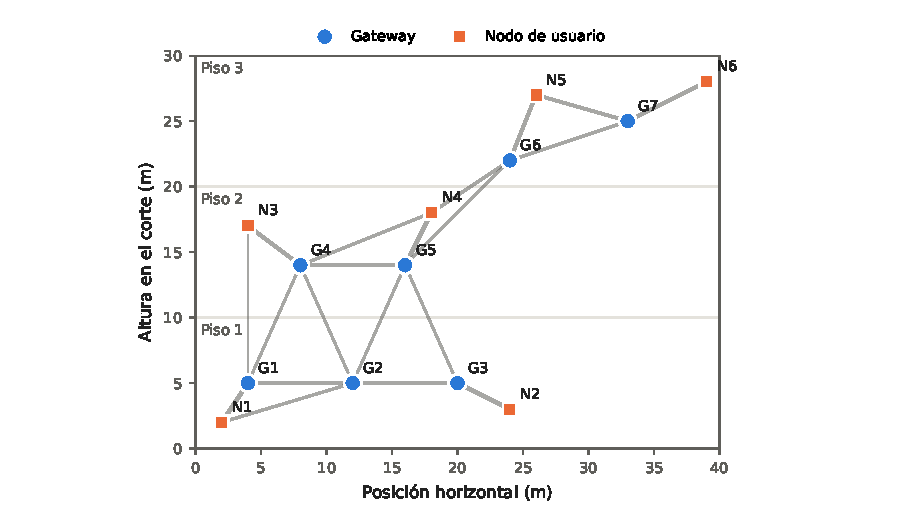
\includegraphics[width=\textwidth]{Images/Cap5/despliegue.pdf}
    \caption{Despliegue de referencia, visto como un corte vertical del edificio de tres pisos. Los círculos son los Gateway (G1 a G7) y los cuadrados, los Nodos de usuario (N1 a N6). Cada línea es un enlace de radio posible entre dos nodos, y su grosor aumenta con la fiabilidad del enlace. G6 es el único enlace entre el piso 3 y el resto}
    \label{fig:despliegue}
\end{figure}

En este despliegue el alcance de radio es de 12~m, la degradación con la
distancia es $\phi=0.5$ y la atenuación por piso es $a_f=0.8$ (estos símbolos se
definen en la Sección~\ref{sec:medio}); representan equipos de baja potencia para
interiores. Se eligieron estos valores en lugar de los valores por defecto del
simulador (Figura~\ref{fig:fiabilidad}) por una razón práctica: con el medio por
defecto, un despliegue con un puente y un borde en este edificio necesita enlaces
tan largos que la entrega baja a 0.32, y las falsas alarmas ocultan los fallos
que se quieren estudiar. Esta elección es un supuesto del experimento y no una
calibración con equipos reales.

\begin{figure}[htbp!]
    \centering
    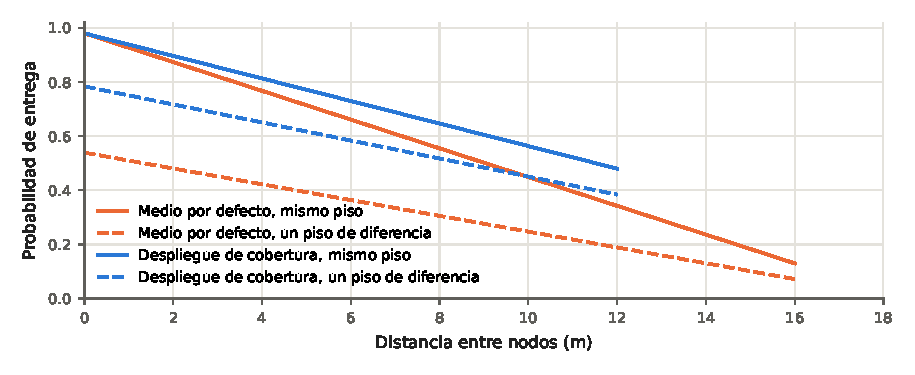
\includegraphics[width=\textwidth]{Images/Cap5/fiabilidad.pdf}
    \caption{Fiabilidad de un enlace, es decir, probabilidad de que una transmisión llegue, según la distancia entre los dos nodos. Se comparan el medio por defecto del simulador y el del despliegue de referencia, para nodos en el mismo piso y con un piso de diferencia. Más allá del alcance la fiabilidad es cero}
    \label{fig:fiabilidad}
\end{figure}

\subsection{Pruebas y corridas}
\label{subsec:experimentos}

Las pruebas son simulaciones. Cada una se define en un archivo de lote del
repositorio, que indica los escenarios, las semillas y la duración. El catálogo
completo, con el nombre, el propósito y el resultado esperado de cada prueba,
está en la Sección~\ref{sec:pruebas}. En total son 45 configuraciones por 10
semillas, es decir, 450 corridas.

Además del despliegue de referencia se usan cinco escenarios heredados del
repositorio base (\texttt{base}, \texttt{colapso\_progresivo},
\texttt{particion}, \texttt{rescatista\_perdido} y \texttt{denso}) para comparar
los modos de movimiento; el nombre \texttt{rescatista\_perdido} se conserva
para poder rastrearlo y designa simplemente a un Gateway que se aleja del
grupo. Los modos de movimiento \textit{seguir} y \textit{repartir} usan
información global a propósito: son la referencia centralizada contra la que se
mide lo que se gana o se pierde al decidir localmente.

\section{Métricas}
\label{sec:metricas}

Cada corrida produce las métricas de la Tabla~\ref{tab:metricas}. Se separan
las que describen la física (qué nodos se pueden conectar por radio) de las que
describen el protocolo o lo que creen los nodos, porque la diferencia entre unas
y otras es justamente lo que se quiere estudiar. La cobertura se mide con la
cobertura media; la adaptabilidad, con el tiempo que la malla pasa partida, el
tiempo que tardan las rutas en rehacerse y la entrega de datos durante y después
de un fallo.

\begin{table}[htbp!]
    \centering
    \caption{Métricas que produce cada corrida y su definición. Un ``componente'' es un grupo de nodos que pueden comunicarse entre sí por radio, directamente o a través de otros}
    \label{tab:metricas}
    \footnotesize
    \begin{tabular}{|p{3.5cm}|p{10.7cm}|}
        \hline
        \textbf{Métrica} & \textbf{Definición} \\
        \hline
        Cobertura media & Promedio en el tiempo de la fracción de Nodos de usuario vivos que están en el mismo componente que algún Gateway vivo \\
        \hline
        Malla partida (s) & Tiempo con los Gateway vivos repartidos en más de un componente. Los enlaces se cuentan entre todos los nodos vivos, de modo que un Nodo de usuario también puede unir dos grupos \\
        \hline
        Reconvergencia de rutas (s) & Tiempo desde que vuelve un Gateway o se reunifica la malla hasta que todo par de Gateway conectados por radio tiene una ruta vigente. ``No aplica'' si no hubo un episodio completo \\
        \hline
        Alertas & Veces en que un Gateway deja de oír a otro durante más del tiempo límite (30~s) \\
        \hline
        TQ medio y saltos medios & Promedios sobre las rutas de las tablas de todos los nodos vivos \\
        \hline
        Tasa de entrega del radio & Transmisiones entregadas sobre intentadas por el medio \\
        \hline
        Entrega de datos & Paquetes entregados sobre enviados, llevados por las tablas de rutas \\
        \hline
        Entrega con camino & Lo mismo, contando solo los paquetes cuyo destino estaba vivo y tenía algún camino por radio al enviarse. Separa el enrutamiento de la física \\
        \hline
        Estiramiento & Saltos recorridos sobre saltos del camino más corto por radio al enviar \\
        \hline
        Causas de pérdida & Fracción de los paquetes que se perdió por cada causa: sin camino por radio, sin ruta, ruta vieja, salto perdido por el radio o bucle \\
        \hline
        Transmisiones por paquete & Intentos de envío por cada paquete de datos. No incluye los mensajes de control del protocolo \\
        \hline
        Exactitud del conocimiento & Fracción de pares ordenados $(a,b)$ de nodos vivos en que $a$ cree lo correcto: tiene ruta vigente hacia $b$ si y solo si el radio los conecta \\
        \hline
        Rutas fantasma y faltantes & Fracción de pares con ruta vigente pero sin conexión por radio, y con conexión por radio pero sin ruta vigente \\
        \hline
        Nodos críticos & Promedio en el tiempo del número de nodos cuya caída partiría la red \\
        \hline
    \end{tabular}
\end{table}

\section{Análisis estadístico}
\label{sec:analisis-estadistico}

El simulador usa números al azar, por ejemplo para decidir si una transmisión
llega. La \textit{semilla} es el valor con el que arranca el generador de esos
números: con la misma semilla y la misma configuración se repite exactamente la
misma corrida. Cada configuración se corre con 10 semillas (1 a 10) y se reporta
como media $\pm$ desviación estándar. Las métricas que no aplican en una corrida
no entran en el promedio.

Para comparar dos configuraciones se usan diferencias pareadas por
semilla~\cite{Jain1991Art}: para cada semilla se resta el resultado de las dos
configuraciones, y con esas diferencias se construye el intervalo de confianza
de la Ecuación~(\ref{eq:ic}):
\begin{equation}
\label{eq:ic}
\bar{D} \;\pm\; t_{0.975,\,n-1}\,\frac{s_D}{\sqrt{n}},
\end{equation}
donde $n$ es el número de semillas (10); $\bar{D}$ es el promedio de las $n$
diferencias; $s_D$ es su desviación estándar, y $t_{0.975,\,n-1}$ es el valor de
la distribución $t$ de Student con $n-1$ grados de libertad que deja el 95~\% de
la probabilidad en el centro (2.262 para $n=10$). Si el intervalo no contiene el
cero, la diferencia se considera concluyente.

Comparar con la misma semilla reduce la variación debida al azar, pero no la
elimina, porque las corridas se separan en cuanto cambia la configuración. No se
aplica corrección por hacer varias comparaciones, de modo que un intervalo que
excluye el cero por poco debe leerse como un indicio y no como una prueba. Con
10 semillas tampoco se comprueba que las diferencias sigan una distribución
normal.

\section{Cómo se comprueba el simulador}
\label{sec:verificacion}

El simulador se comprueba de cuatro maneras:

\begin{itemize}
\item \textbf{Pruebas de simulación:} escenarios con un resultado esperado, que
se comparan con lo que el simulador produce (Sección~\ref{sec:pruebas}).
\item \textbf{Cálculo a mano:} cuando una métrica se puede calcular a partir del
escenario, se compara con la simulación (Sección~\ref{sec:res-verificacion}).
\item \textbf{Repetibilidad:} la misma semilla y la misma configuración deben
dar la misma corrida, también entre la terminal y la interfaz web y entre
computadores distintos.
\item \textbf{Comprobaciones automáticas del código:} un conjunto de
verificaciones que se ejecuta con una orden y avisa si un cambio rompió algo
(Anexo B).
\end{itemize}

\section{Amenazas a la validez}
\label{sec:amenazas}

\textbf{Lo que se mide.} La cobertura se define como estar en el mismo
componente de radio que algún Gateway, lo que no garantiza un enlace de buena
calidad ni que exista una ruta en las tablas. Por eso se reporta junto a la
entrega de datos.

\textbf{Decisiones de los autores.} Hay valores elegidos por los autores: los
umbrales del movimiento descentralizado salieron de una búsqueda sobre cuatro
de los escenarios en los que luego se compara, y eso favorece a ese modo. El
despliegue de referencia se diseñó para tener puentes y bordes, de modo que no
representa a un despliegue típico.

\textbf{Generalización.} El modelo del medio es simple y simétrico, sin
colisiones ni cambios en el tiempo, supuestos que la literatura ha mostrado
optimistas~\cite{Kotz2004Assumptions}. Por ello, las magnitudes absolutas no se
trasladan a un despliegue físico, aunque las comparaciones relativas sí sirven
para orientar hipótesis.

\textbf{Conclusiones estadísticas.} Diez semillas dan intervalos amplios en las
métricas más variables. En algunas tablas un solo caso domina la dispersión,
como se señala al discutirlas.
